% QUESTAO
Um quadro tem forma retangular de dimensões externas $60\times 40$\,cm. A moldura tem largura $x$ uniforme. Calcule a largura, sabendo que a área da tela é $1196$\,cm$^2$.
\begin{center}
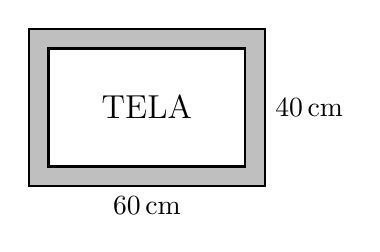
\begin{tikzpicture}[scale=0.500000,thick]
\draw[fill=gray!50] (0,0) rectangle (6,4);
\draw               (0,0) rectangle (6,4);
\node[below] at (3.0, 0  ) {$60$\,cm};
\node[right] at (6  ,2.0) {$40$\,cm};
\draw[thick,fill=gray!0] (0.5,0.5) rectangle (5.5,3.5);
\node at (3.0,2.0) {\large TELA};
\end{tikzpicture}
\end{center}

% ALTERNATIVAS 7
$x=7$\,cm
$x=8$\,cm
$x=6$\,cm
$x=4$\,cm
$x=5$\,cm



